% This is the aspauthor.tex LaTeX file
% Copyright 2010, Astronomical Society of the Pacific Conference Series

\documentclass[11pt,twoside]{article}
\usepackage{asp2010}

\resetcounters

\bibliographystyle{asp2010}

\markboth{Economou et al.}{Lessons learned from NDF}

\newcommand{\aspconf}{ASP Conf.\ Ser.}

\begin{document}

\title{Advantages of extensible self-described data formats: Lessons learned from NDF}
\author{Frossie~Economou$^1$, Tim~Jenness$^2$, Malcolm~J.~Currie$^3$,
and David~S.~Berry$^3$
\affil{$^1$National Optical Astronomy Observatory, 950 N.\ Cherry Ave,
Tucson, AZ 85719, USA}
\affil{$^2$Department of Astronomy, Cornell University, Ithaca, NY
  14853, USA}
\affil{$^3$Joint Astronomy Centre, 660 N.\ A`oh\=ok\=u Place, Hilo, HI
96720, USA}
}

\begin{abstract}
  In the context of current discussions about the future of data
  formats, we present an overview of key features of the NDF
  format. In our experience, these features offer advantages for
  archive-side reprocessing and publication of data products, and
  provide valuable lessons learned for future data format designers.
\end{abstract}

\section{Introduction}

The extensible $N$-Dimensional Data Format
\citep[NDF;][]{1993ASPC...52..229W,SGP38} was a data model layered on
top of the Starlink (ascl:1110.012) Hierarchical Data System
\citep[HDS;][]{1982QJRAS..23..485D}. During the 1980s it became clear
that a general hierarchical file format without regard for conventions
was a recipe for incompatibility and confusion \citep[see
e.g.][]{1993ASPC...52..219S}. NDF was developed in response to this
issue and was released in 1987 \citep[see
e.g.][]{1988STARB...2...11C}.

NDF contains standardised conventions for representing data,
variance and quality masks, handling history and provenance, along
with a data-access library that can support data sectioning, including
WCS slices. Over the years the format has been extended to support
world-coordinate objects \citep{2001ASPC..238..129B}, data compression
\citep{2008ASPC..394..650C} and provenance tracking
\citep{2009ASPC..411..418J}.

\section{Facilities of the HDS Data Format}

NDF is designed such that it can make use of the hierarchical
organization of primitives and structures supported by HDS. HDS can
store arrays of numbers and strings, structures containing other
structures and also arrays of structures. This means, for example,
that an HDS file can itself contain multiple structures of type
NDF. This facility is very useful for acquisition systems that have
multiple readouts.

\section{Components of the NDF Data Model}

In this section we provide a general overview of the data model
implemented by NDF.

\subsection{Data, Variance, and Quality}

Data arrays, variance components and quality masks are all grouped
into \texttt{ARRAY} structures which also support the the creation of
cut-outs that retain knowledge of their origin within a wider pixel
coordinate system.  Along with these $N$-dimensional array components,
title, data label and data units are explicitly supported metadata.

A mask array is available to allow each pixel in the main data array
to be associated with a particular quality. NDF supports up to 8 bits
of quality, and the bits can be associated with easy-to-remember
string labels, and the individual bits can be activated based on a bit
mask applicable to the whole array. Additionally, it is possible to
use magic ``bad'' values where data is known to be irrevocably bad
regardless of quality settings.

\subsection{World Coordinates}

World Coordinates are handled by storing a serialized WCS object
generated by the AST library \citep{1998ASPC..145...41W}. AST provides
a flexible system that allows multiple coordinate frames to be
connected using complex mappings formed by stacking simple atomic
mappings in an arbitrary way. It also has facilities for importing the
full range of FITS-WCS standards \citep[see
e.g.][]{2006A&A...446..747G,2012ASPC..461..825B} into this form,
including support of irregularly sampled or sparse data.

\subsection{History and Provenance}

Rather than being unstructured comment fields, NDF stores history
metadata in explicit data structures with a supporting API. The
history tracks the date, the application name, the user running the
application and the command parameters. Most applications copy history
from a nominated primary input NDF to the output NDF, adding a new
record to describe the application used.

Provenance (determining which files contributed to each step in the
history) can be tracked automatically, by determining which files were
opened by the application, or by explicitly noting which files are
relevant to the output provenance. Unlike History, applications copy
provenance from from \emph{all} input NDFs to the output
NDF. Provenance tracking is critical for archive processing where a
scientist downloading a product should be able to determine which
observations went into the product and enables them to regenerate it
if so desired. An example of a simple, automatically generated,
provenance report is shown in Fig.\ \ref{fig:P91_f1}. The Canadian
Astronomy Data Centre includes provenance in their archive data model
\citep[CAOM;][]{2012ASPC..461..339D,2013ASPC..475..159R}, and the data
pipeline for the JCMT Science Archive \citep{2008ASPC..394..565J} was
able to include provenance information in its products without
requiring extensive instrument-specific modifications.

\begin{figure}
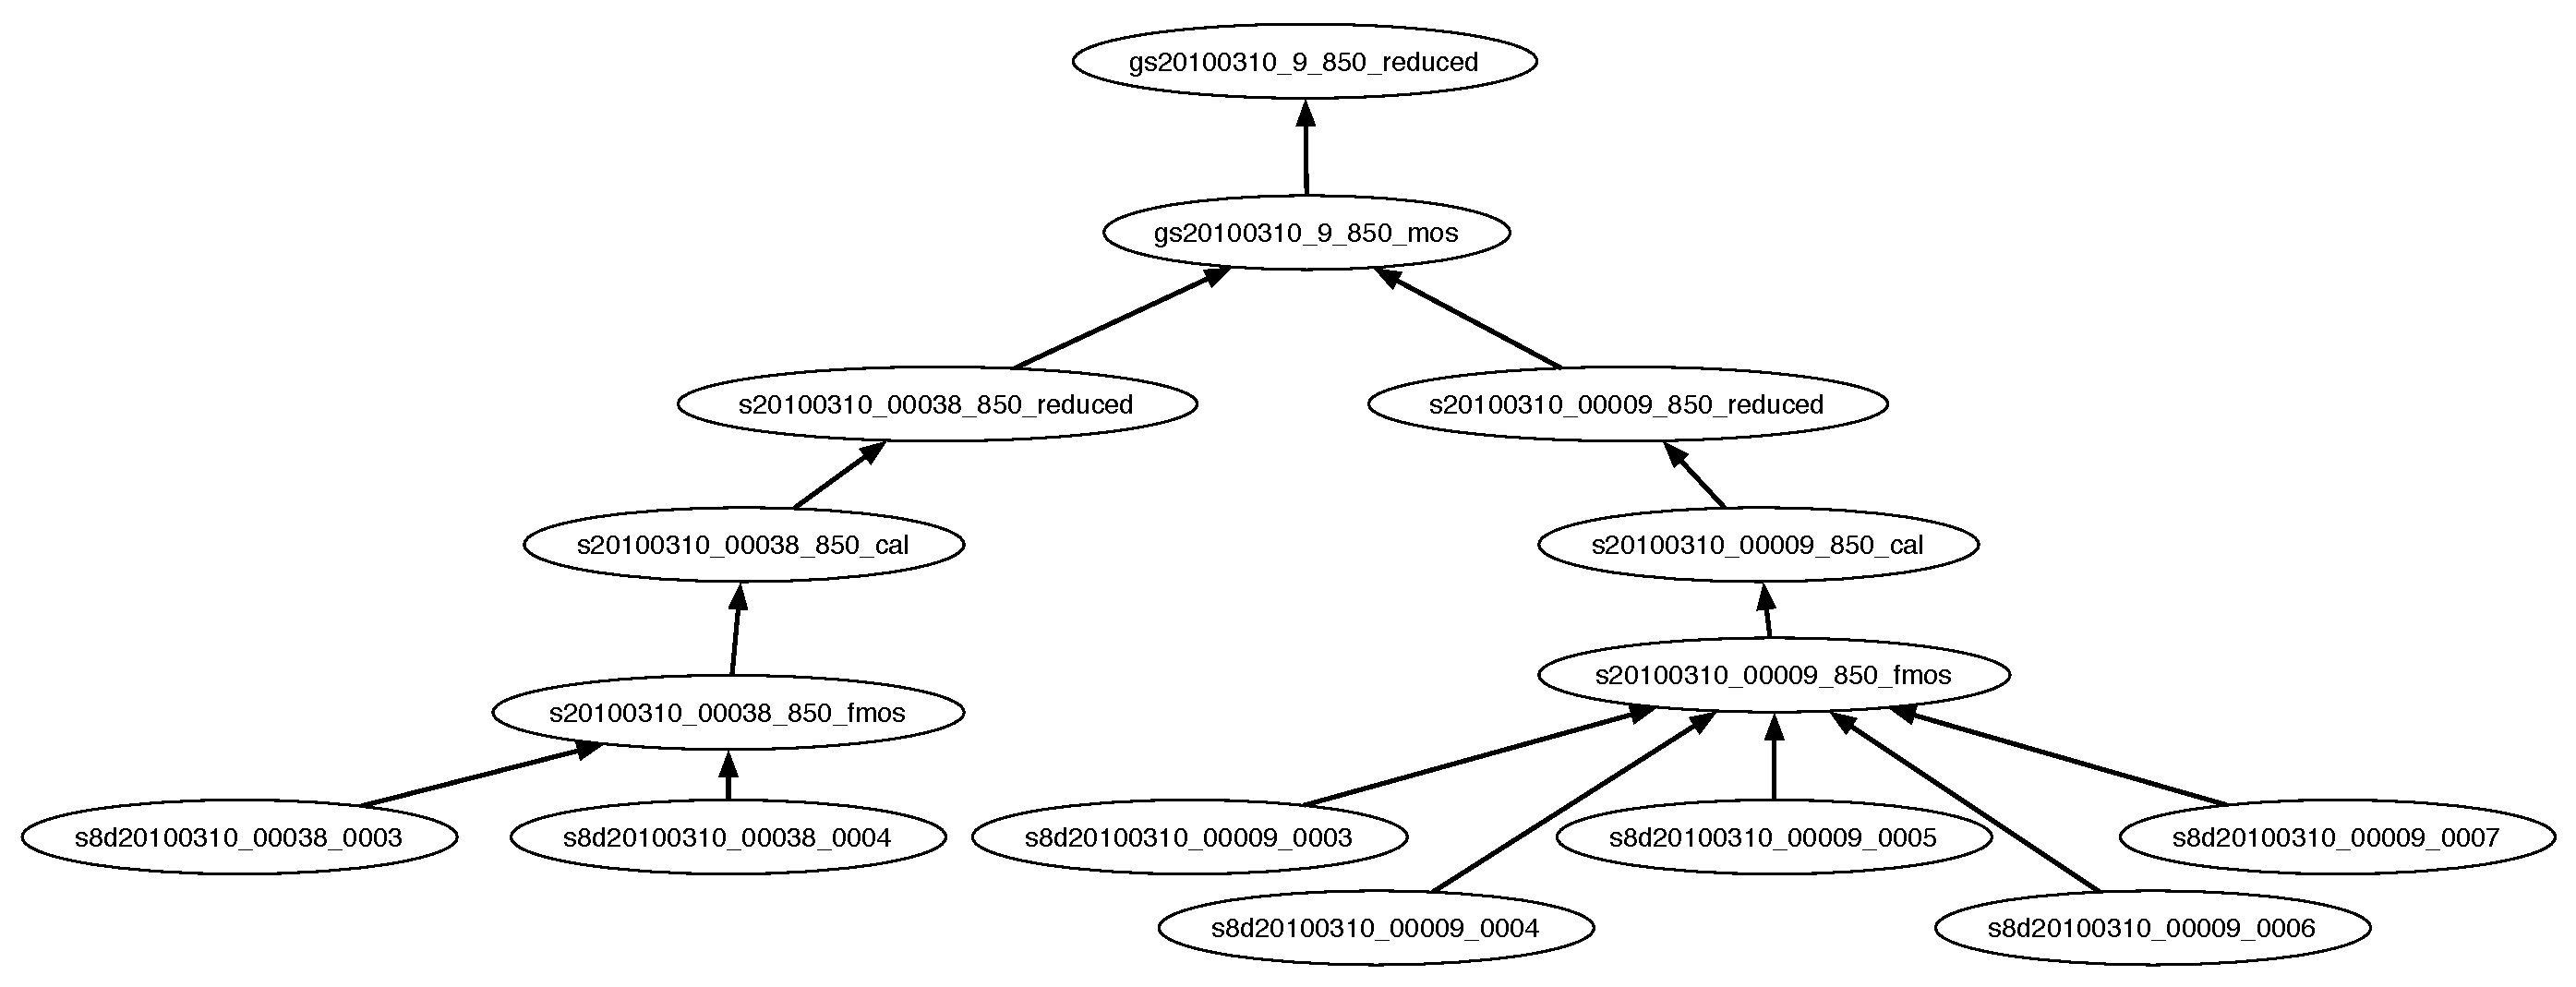
\includegraphics[width=\textwidth]{P91_f1}
\caption{Provenance diagram for a data product consisting of seven raw
  data files spread over two observations and three intermediate steps.}
\label{fig:P91_f1}
\end{figure}

\subsection{Extensions}

Arbitrary structures can be stored in the \texttt{MORE}
extension. Extensions can be HDS structures but it's recommended that
where possible NDFs are used to represent array data. For example, the
SMURF application includes an NDF structure representing the effective
exposure time seen by each pixel in its extension. NDF applications
can address structures at any position in the file structure. A SMURF
exposure time image can be displayed by referring to
\texttt{file.MORE.SMURF.EXP\_TIME}. Software packages are free to
define their own structures on the understanding that packages that do
not understand will still propagate the structures during processing.

General keyword/value headers are stored in the extension as an array of
80-character FITS headers. This was a pragmatic decision and ensures
easy compatibility with FITS header parsers and conversion of NDF to
and from FITS.

\section{Lessons Learned}

The developers of NDF were aiming for a general-purpose astronomical
data format suitable for use across multiple wavelength ranges. They
therefore had to provide features that were genuinely useful without
bloating the specification with features demanded by a niche
community.

Over 25 years of use, the NDF approach to a structured data model has
succeeded in its aim of supporting a rich suite of data reduction and
analysis tools in a consistent manner. It has also proven to be
possible to round-trip to FITS files without losing the complex
organizational structure \citep[see e.g.][]{1997STARB..19...14C}. It
is hoped that these lessons can feed into discussions on the future
direction of FITS as espoused in \citet{P90_adassxxiii}.

A few lessons have been learned from experience with using NDF. It
became clear that restricting quality to only 8 bits was not a
sustainable solution and a flexible bit count is required. Software
such as the SMURF package \citep{2013MNRAS.430.2545C} now make use of
16-bit quality internally and have to combine bits when exporting to
NDF. Additionally, there was a tendency early on to create overly
complex application-specific extensions rather than trying to re-use
more widely understood structures. Variance is a useful way of
representing an error but there is demand for support of different
error schemes. Finally, the lack of native table support in HDS
(something added to FITS \citep{1988A&AS...73..365H} whilst NDF was
being developed) has restricted the applicability of NDF for some
applications.

\bibliography{P91}

\end{document}
